\documentclass[11pt]{article}

\usepackage[margin=1in]{geometry}
\usepackage{graphicx}
\usepackage{booktabs}
\usepackage{tabularx}
\usepackage{array}
\usepackage{enumitem}
\usepackage{hyperref}
\usepackage{xcolor}
\usepackage{tikz}
\usepackage{subcaption}
\usepackage{fancyhdr}
\usepackage{float}
\usepackage{setspace}

\usetikzlibrary{arrows.meta, positioning, shapes.geometric}

\definecolor{deadred}{HTML}{A12F2F}
\definecolor{deadgold}{HTML}{B88B2A}
\definecolor{deadink}{HTML}{1D1D1D}
\definecolor{deadgray}{HTML}{5E5E5E}
\definecolor{deadlight}{HTML}{F6F3EE}

\hypersetup{
  colorlinks=true,
  linkcolor=deadred,
  urlcolor=deadred,
  pdftitle={Deadlight Deliverable 2 Mid-Project Report},
  pdfauthor={Group 16}
}

\pagestyle{fancy}
\fancyhf{}
\lhead{Deadlight Deliverable 2}
\rhead{Group 16}
\cfoot{\thepage}
\setlength{\headheight}{14pt}

\setstretch{1.08}
\setlength{\parindent}{0pt}
\setlength{\parskip}{0.55em}
\setlist[itemize]{leftmargin=1.4em, itemsep=0.3em, topsep=0.35em}
\setlength{\emergencystretch}{2em}
\captionsetup{font=small, labelfont=bf}

\newcolumntype{Y}{>{\raggedright\arraybackslash}X}

\begin{document}
\pagenumbering{gobble}
\hypersetup{pageanchor=false}

\begin{titlepage}
    \centering
    \vspace*{1.2cm}

    {\Large CS4483B / 9541 Game Design \par}
    \vspace{0.6cm}
    {\Huge \bfseries Deadlight: Survival After Dark \par}
    \vspace{0.35cm}
    {\LARGE Deliverable 2 Mid-Project Report \par}
    \vspace{0.8cm}

    {\large Group 16 \par}
    \vspace{0.2cm}
    {\normalsize
    Simranjeet Singh \\
    Abdelrahman El Banna \\
    Koroush Emari \\
    Ashraf Esam Mahdi \par}

    \vspace{1.0cm}

    \begin{tabular}{rl}
        \textbf{Submission Scope:} & Deliverable 2 playable prototype covering Levels 1-2 \\
        \textbf{Playable Length:} & Six objective nights across two campaign spaces \\
        \textbf{Project Type:} & Top-down zombie survival prototype in Unity \\
        \textbf{Report Focus:} & Level design, guidance, narrative, systems, progression, and iteration
    \end{tabular}

    \vfill

    \begin{figure}[H]
        \centering
        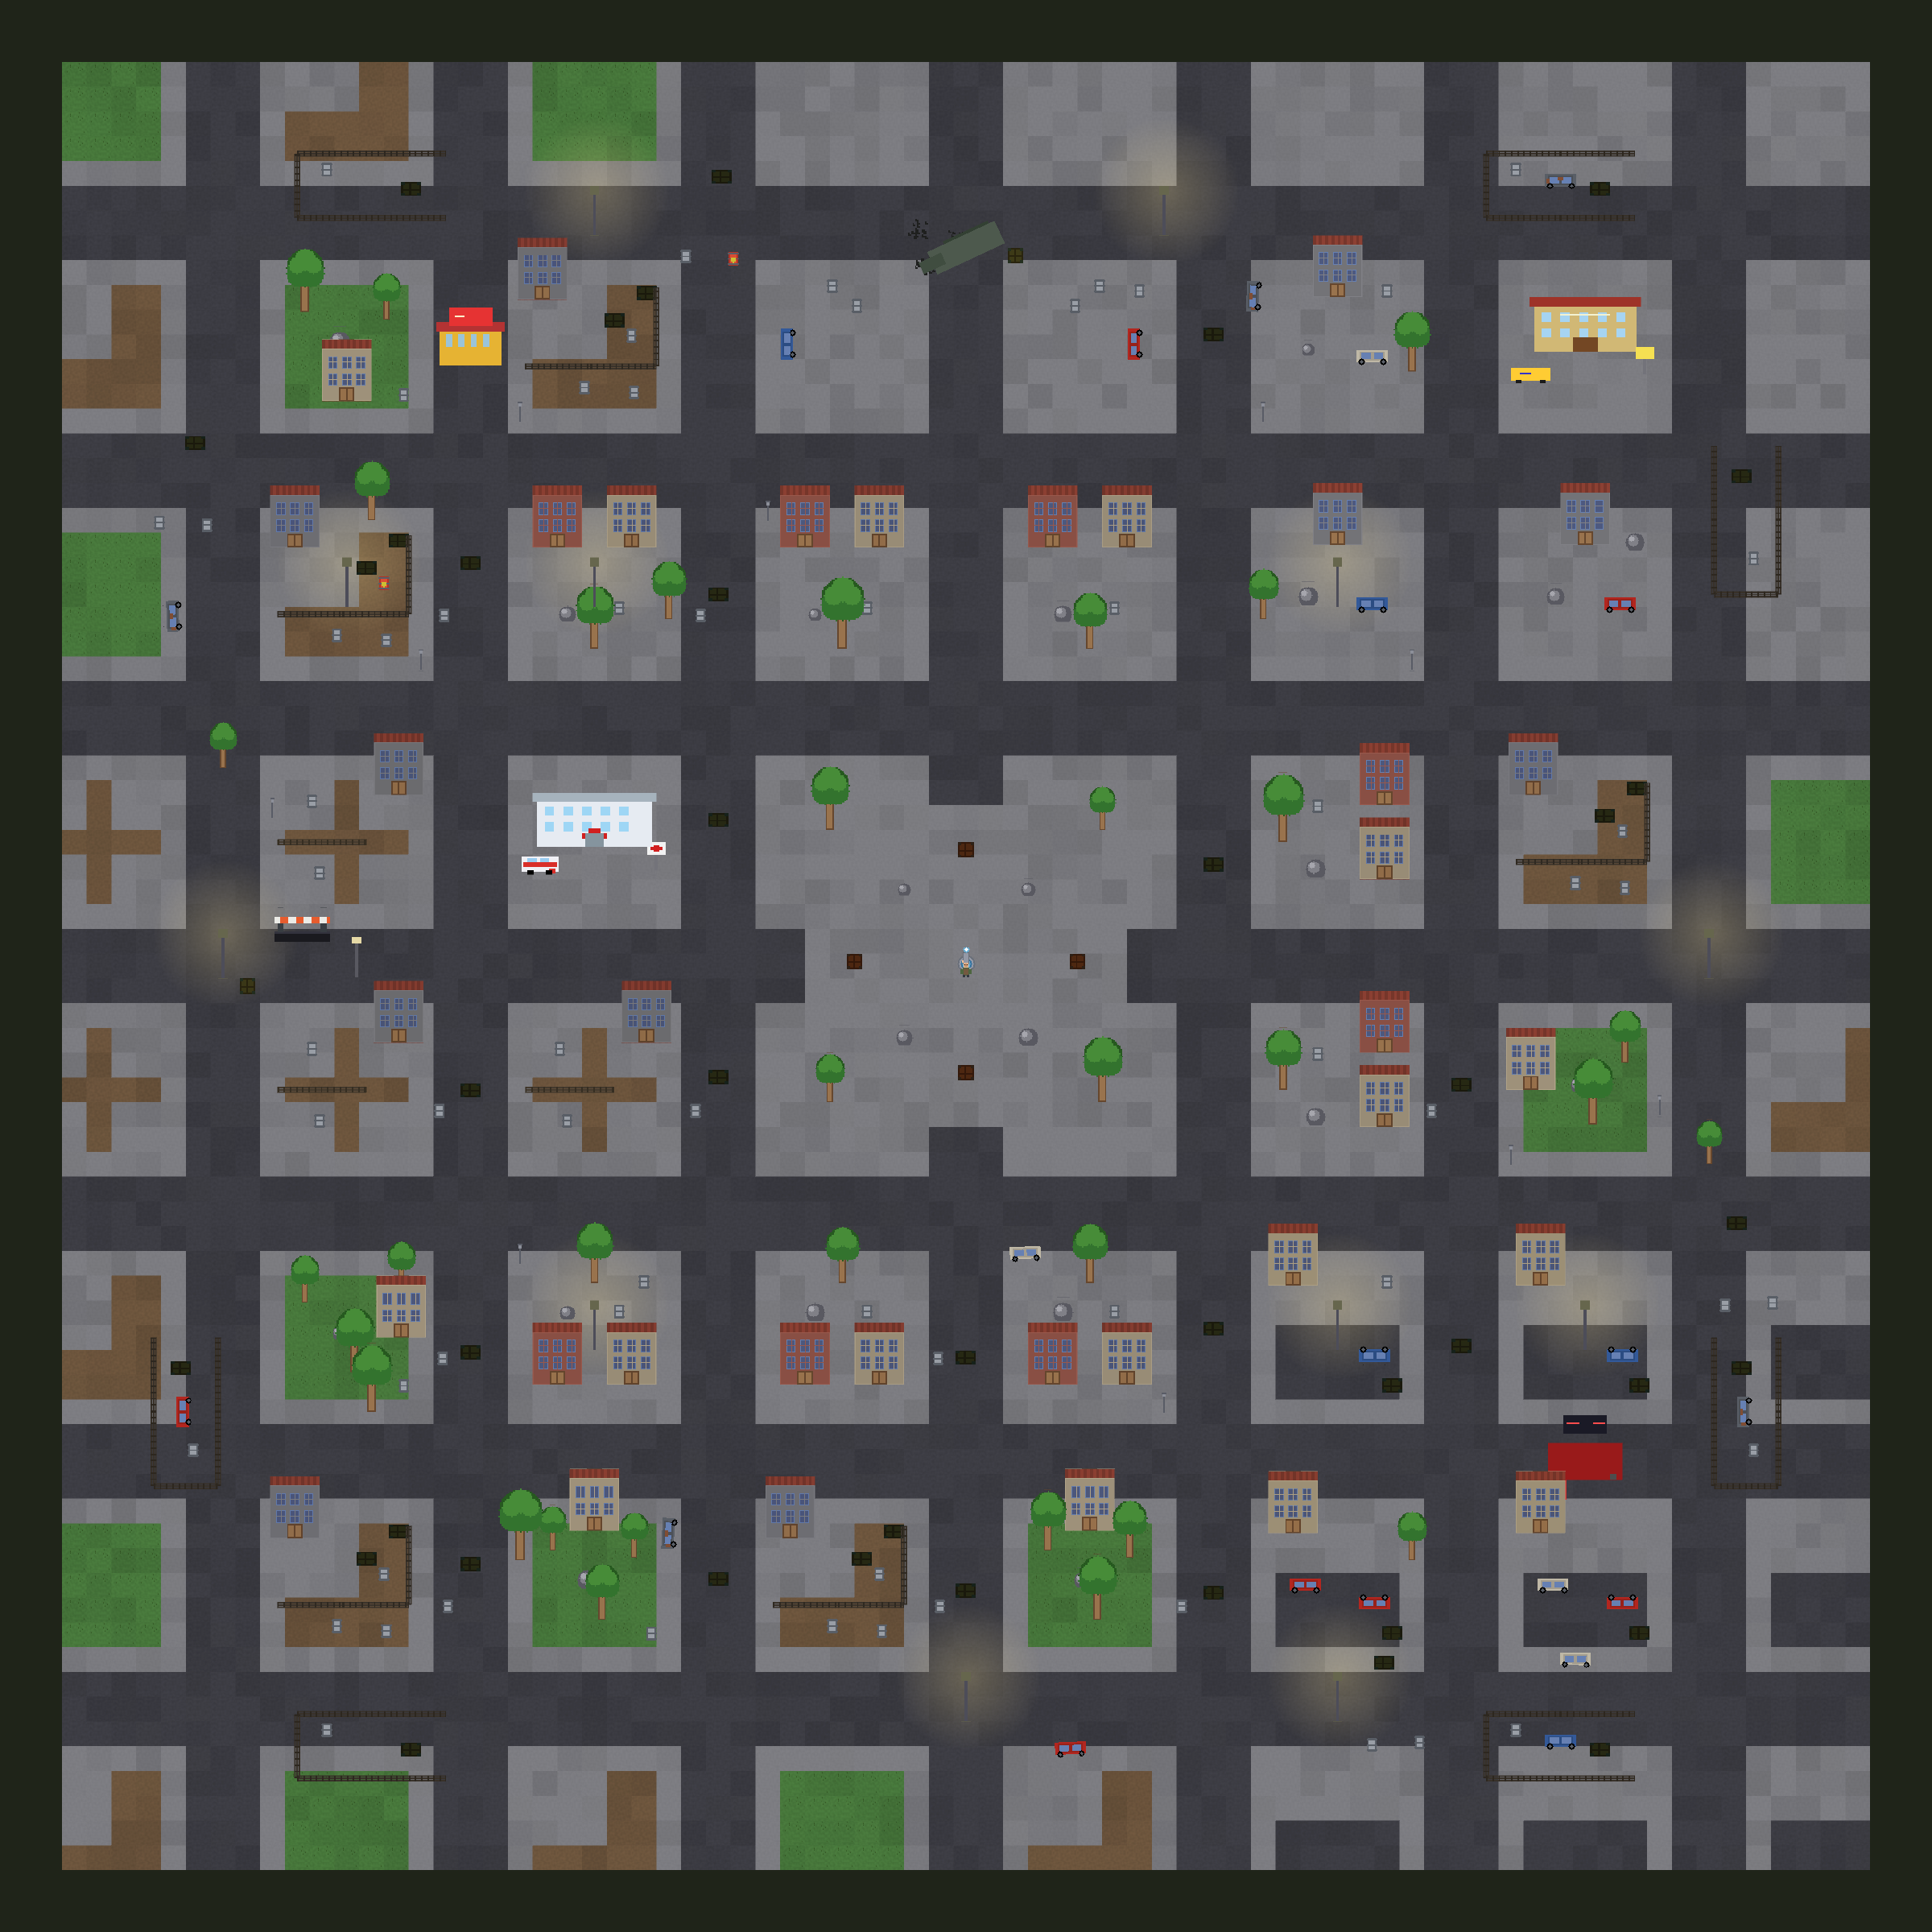
\includegraphics[width=0.74\textwidth]{../Assets/Resources/MenuPreviews/TownCenter.png}
    \end{figure}

    \vfill

    {\large April 2026\par}
\end{titlepage}
\clearpage
\hypersetup{pageanchor=true}
\pagenumbering{arabic}
\setcounter{page}{1}

\section{Project Overview}

Deliverable 2 presents a playable prototype of \textit{Deadlight} in a more complete and structured form than the initial concept build. The current submission focuses on Levels 1 and 2 only, which together form a six-night campaign segment. This scope was selected to provide a clear vertical slice of the intended game while keeping the project manageable for the current stage of development.

The core gameplay loop is organized into three phases. During the day, the player explores the environment, follows objectives, and prepares for the next attack. At night, the player must survive waves of zombies under increasing pressure. At dawn, the player receives points and rewards, then uses the shop to purchase weapons, armor, ammunition, healing items, and upgrades before continuing the run. This structure gives the prototype a clear rhythm and helps connect exploration, combat, and progression into one consistent experience.

The main design goal for this deliverable was to make preparation matter. In earlier versions, the daytime phase risked feeling like a simple break between combat segments. In the current build, player choices during the day have more visible consequences at night through objective rewards, contested drops, and resource management. At the same time, the project places greater emphasis on narrative context through radio transmissions, environmental storytelling, and mission-based progression tied to EVAC Command, Project Lazarus, Dr. Chen, and Subject 23.

\begin{figure}[H]
    \centering
    \begin{subfigure}[t]{0.48\textwidth}
        \centering
        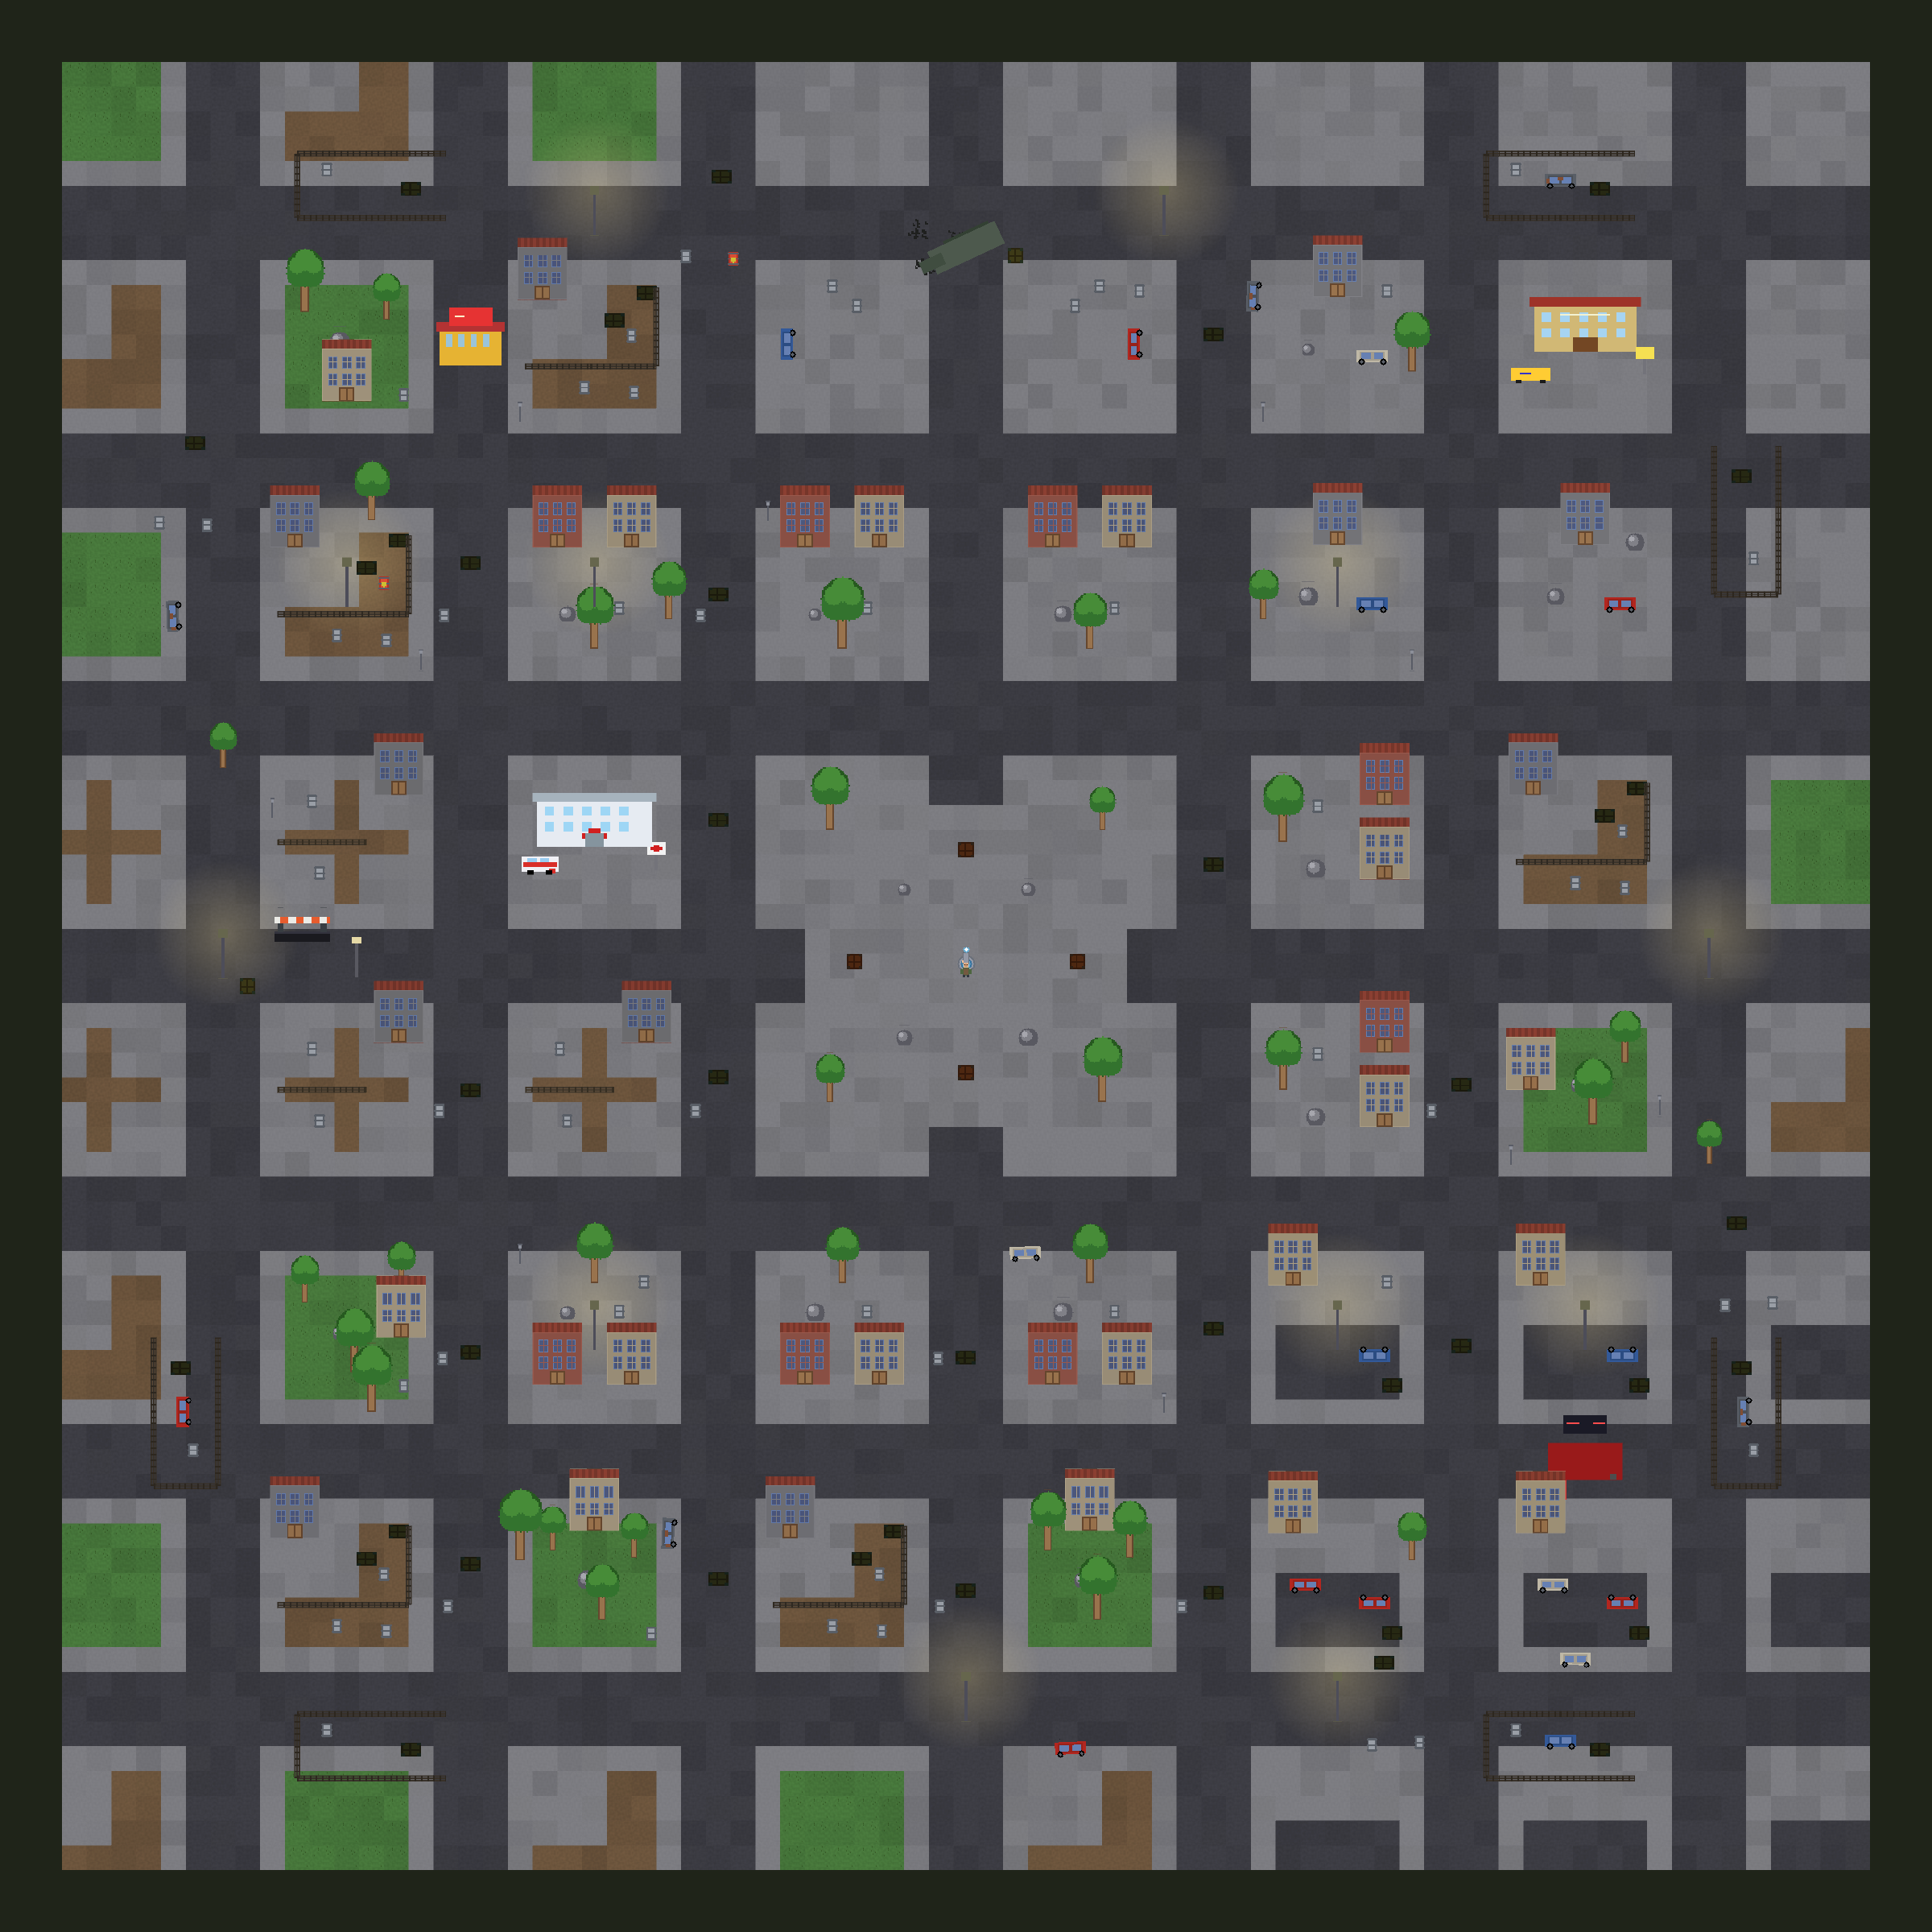
\includegraphics[width=\linewidth]{../Assets/Resources/MenuPreviews/TownCenter.png}
        \caption{Level 1: Town Center. This area introduces the main objective route, early landmarks, and the first three day-night cycles.}
    \end{subfigure}
    \hfill
    \begin{subfigure}[t]{0.48\textwidth}
        \centering
        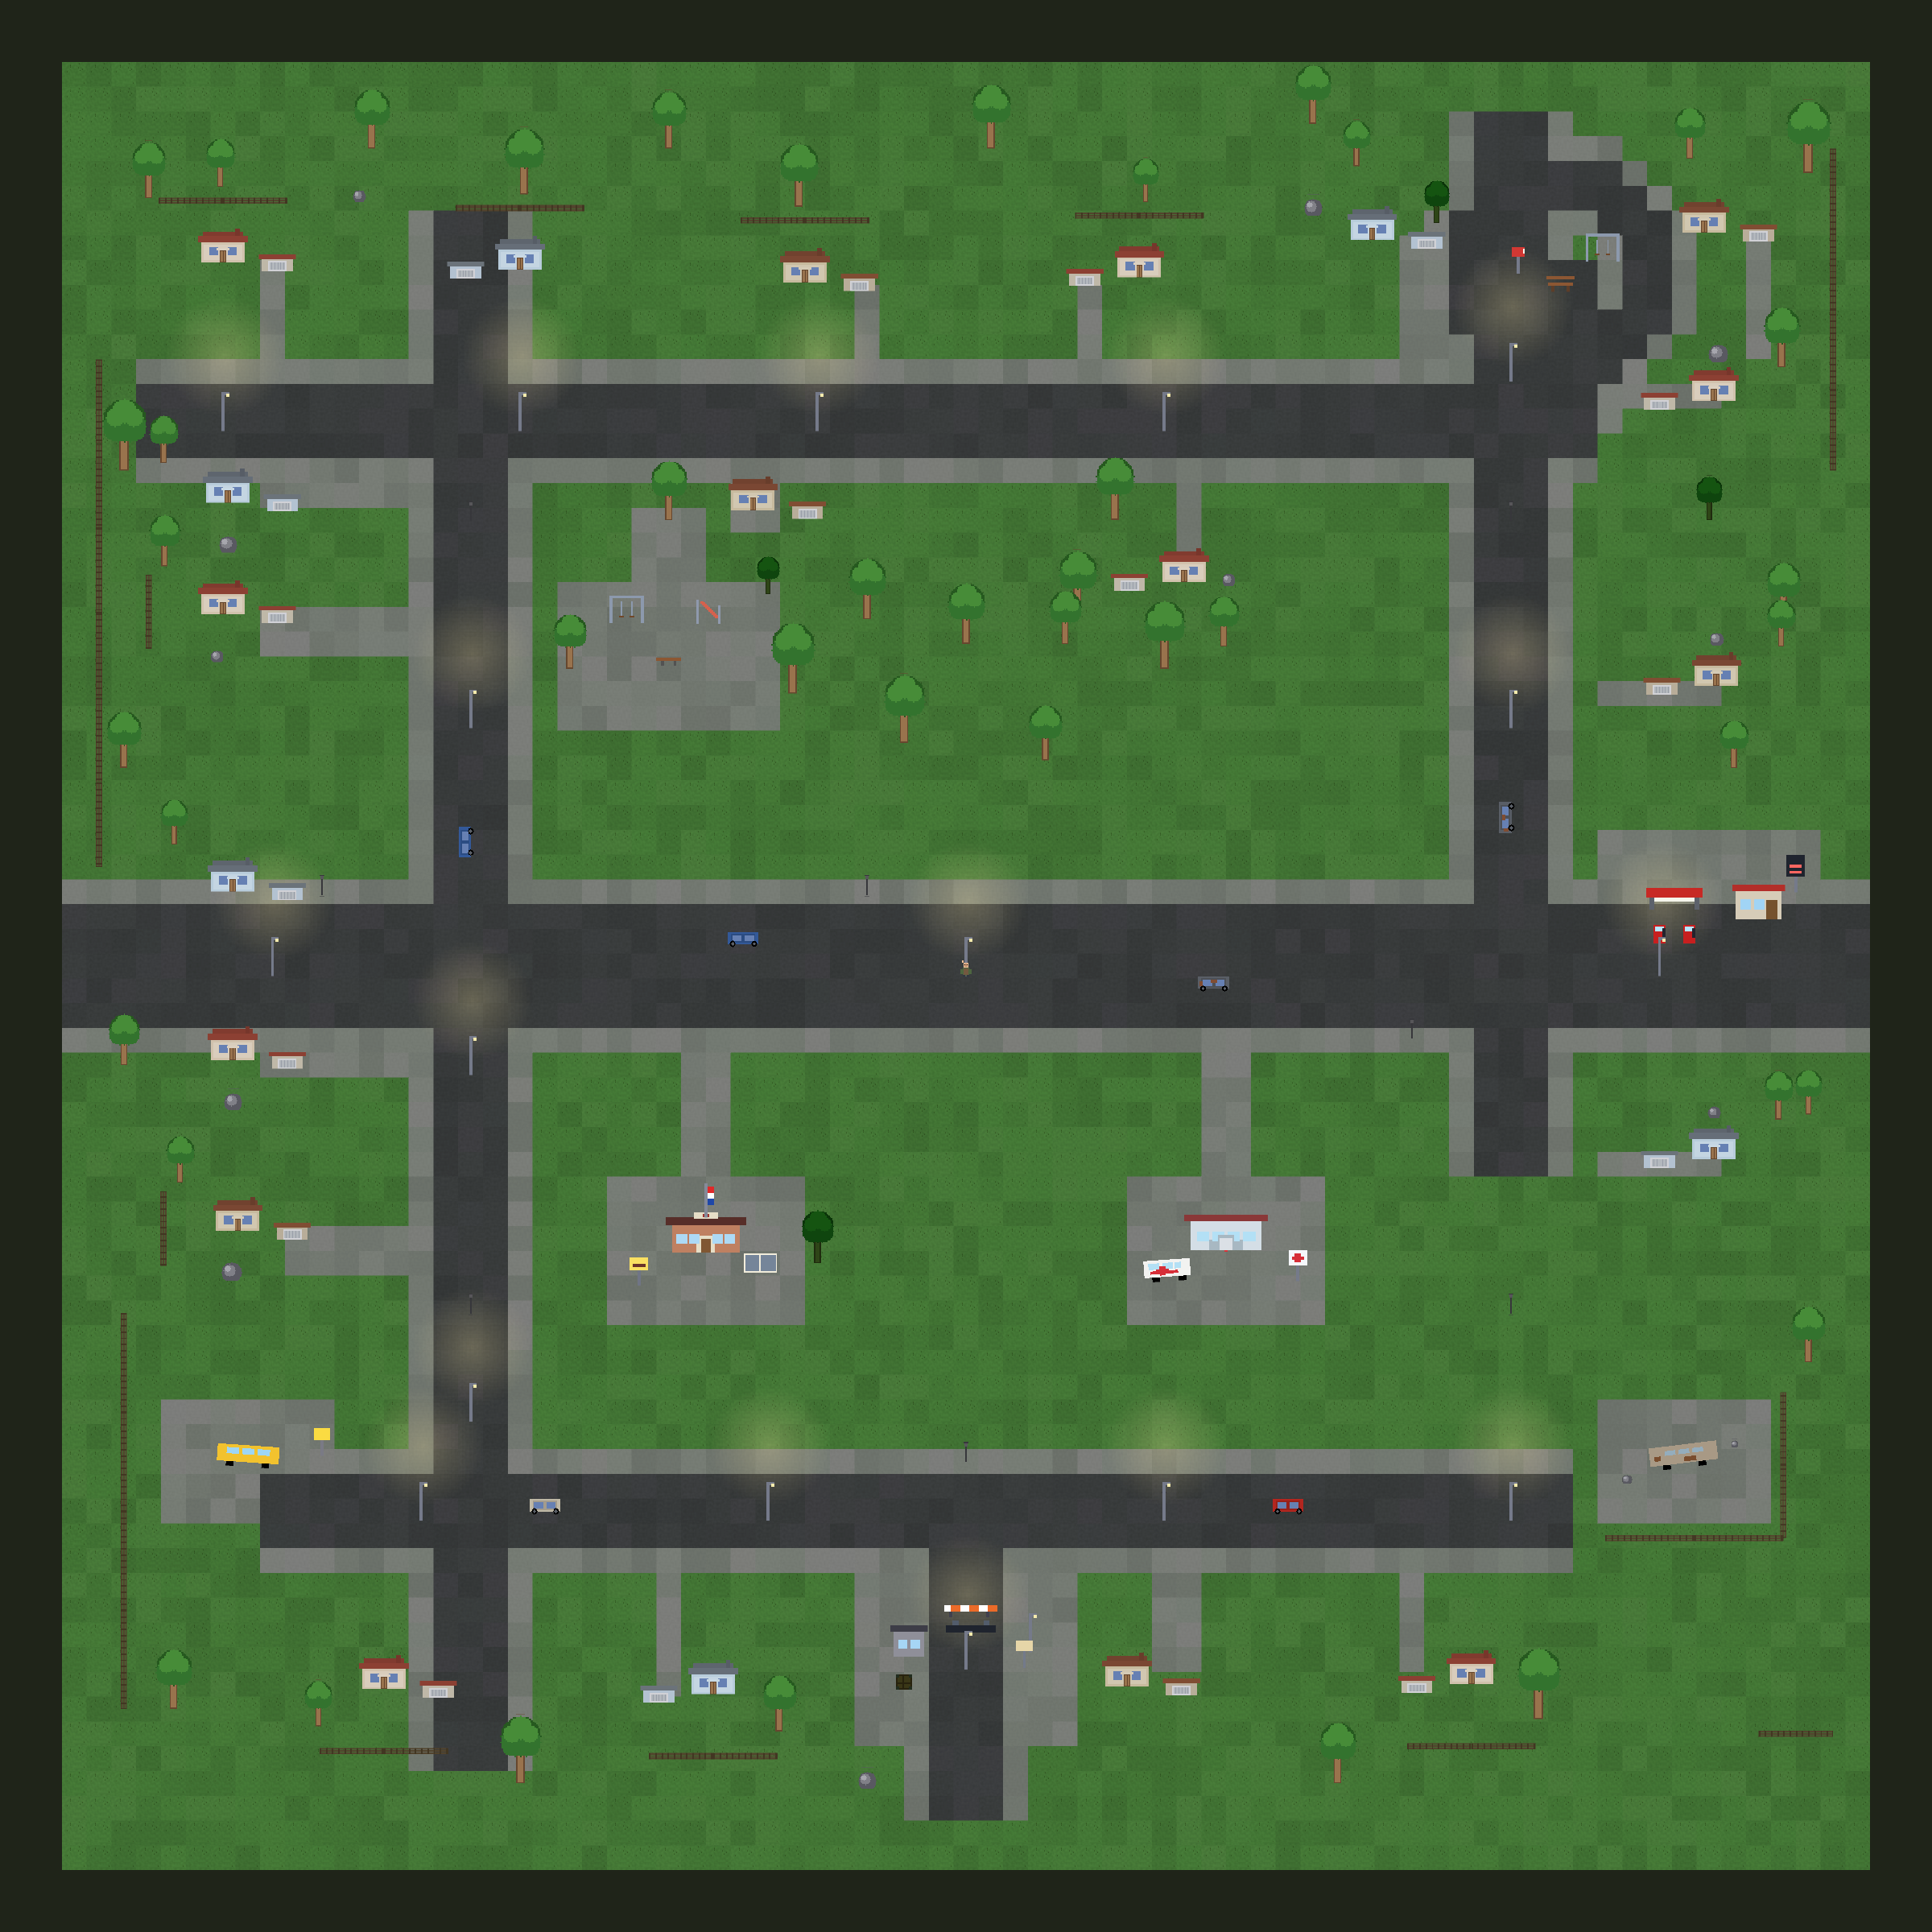
\includegraphics[width=\linewidth]{../Assets/Resources/MenuPreviews/Suburban.png}
        \caption{Level 2: Suburban district. This area expands the route, increases pressure, and continues the campaign.}
    \end{subfigure}
    \caption{Playable Deliverable 2 route. The current prototype intentionally focuses on Levels 1 and 2, while later areas are reserved for future deliverables.}
\end{figure}

\section{Deliverable 2 Criteria Coverage (Point-by-Point)}

\begin{table}[H]
    \centering
    \small
    \begin{tabularx}{\textwidth}{>{\bfseries}p{0.26\textwidth} Y Y}
        \toprule
        Rubric Point & What Is Implemented in the Prototype & How It Is Demonstrated In-Game \\
        \midrule
        Level design and player guidance &
        Two authored spaces (Town Center and Suburban) with route structure, landmark sequencing, and objective-based navigation. &
        Objective HUD + world markers + mission callouts direct movement while preserving optional exploration paths. \\
        Narrative and world-building &
        Mission-aligned radio beats, story objectives, lore pickups, and start/end framing tied to the Lazarus arc. &
        Each night advances plot context (evac failure, quarantine intent, Lazarus evidence) instead of isolated wave survival. \\
        Systems and game balance &
        Day-night-dawn loop with connected economy (points, ammo, health, armor, utility, upgrades), plus escalation by night. &
        Better day execution produces stronger night readiness; weak preparation produces measurable combat pressure. \\
        Progression and rewards &
        Six-night campaign slice with unlock-based level access, reward pacing, and level-specific challenge identity. &
        Level 2 unlocks after Level 1 completion; player manually selects the next deployment from menu for clear control. \\
        Testing and iteration &
        Iterative tuning from playtest feedback and PlayMode validation around objective flow, pickup clarity, and phase transitions. &
        UI callouts, objective readability, and communication pacing were revised based on observed confusion points. \\
        \bottomrule
    \end{tabularx}
    \caption{Line-by-line Deliverable 2 coverage summary. Each rubric point is mapped to implemented systems and observable runtime behavior.}
\end{table}

\section{Level Design and Player Guidance}

The level design for Deliverable 2 aims to guide the player clearly while still allowing exploration. Rather than relying only on direct tutorial text, the prototype uses route structure, landmarks, mission prompts, and pacing changes to communicate where the player should go and what they should do next.

Level 1 serves as the introduction to the playable campaign. Its route moves the player through major landmarks such as the crash site, the military checkpoint, and the hospital. These locations are intentionally distinct so that the player can build a mental map of the area and understand the mission flow without becoming lost. Level 2 continues the same design approach, but the spaces are broader and more exposed. This creates a stronger sense of danger and makes navigation, scavenging, and defensive planning more demanding.

The two levels also support the learning curve of the prototype. Level 1 teaches the structure of exploration, preparation, and survival. Level 2 then asks the player to apply that understanding under greater pressure. This progression is important because it lets the prototype demonstrate not only basic functionality, but also how the game scales over time.

Player guidance is delivered through several overlapping cues:

\begin{itemize}
    \item mission titles and live objective status through the in-game objective HUD,
    \item world-space objective markers that point toward the next important location,
    \item radio transmissions that give short narrative and tactical direction,
    \item recognizable landmarks that help the player build mental maps of each space,
    \item pacing shifts between day exploration and night defense.
\end{itemize}

This combination supports a balance between freedom and clarity. The player can search for resources, optional lore, and useful routes, but the game still signals the next critical task. This is especially important in a survival project, because difficulty should come from decision-making and pressure rather than uncertainty about the objective.

\textbf{Implementation detail by point.}
\begin{itemize}
    \item \textbf{Route readability:} both playable levels are structured around clear lanes, recognizable silhouettes, and mission landmarks so orientation can happen quickly under pressure.
    \item \textbf{Guidance redundancy:} objective title, objective status text, world marker, and radio prompt communicate the same target through different channels.
    \item \textbf{Difficulty through space:} Level 2 introduces wider exposure, longer approach vectors, and less forgiving reposition windows than Level 1.
    \item \textbf{Player agency:} the route is guided but not hard-rail; players can still choose loot order, engagement path, and fallback position.
\end{itemize}

\section{Narrative Design and World-Building}

The narrative design follows a play-first approach. Story information is delivered during movement, scavenging, defense, and mission completion instead of being placed mainly in long cutscenes. This helps the prototype maintain pacing while still giving the player a clear sense of setting, purpose, and escalation.

In the Deliverable 2 build, the player is presented as the survivor of a failed evacuation attempt. Across six nights, the player receives instructions and updates from EVAC Command while moving through two unsafe districts in search of supplies, answers, and a path to extraction. As the campaign progresses, the radio dialogue and mission structure reveal more about Project Lazarus, Dr. Chen, and Subject 23. This gives the run a stronger narrative arc than a simple wave-based survival mode.

We use several layers of narrative delivery:

\begin{itemize}
    \item \textbf{Radio story beats} communicate the broad situation, major discoveries, and rising danger.
    \item \textbf{Story objectives} tie important plot information to specific spaces the player must reach.
    \item \textbf{Lore entries} add optional depth through logs, journals, military orders, and intercepted transmissions.
    \item \textbf{Environmental framing} makes each district feel like a place that was defended, abandoned, and partially erased.
    \item \textbf{Intro and ending sequences} give the playable run a stronger beginning and end-state.
\end{itemize}

This layered approach improves immersion because the main story remains understandable even if the player only follows core objectives, while optional exploration still provides additional depth. It also helps the prototype feel more unified. The player's goals, the spaces they move through, and the systems they interact with all support the same survival narrative.

\textbf{Implementation detail by point.}
\begin{itemize}
    \item \textbf{Narrative pacing:} story information is distributed across mission beats so context arrives before, during, and after pressure spikes.
    \item \textbf{Character channel clarity:} EVAC Command, field voice, and intercept-style lines are used with distinct wording and timing roles.
    \item \textbf{World coherence:} objective locations and environmental context are aligned so story events happen in spaces that logically support them (crash site, checkpoint, clinic/shelter chain).
    \item \textbf{Optional depth:} lore collection is additive and does not block core progression, preserving readability for first-time players.
\end{itemize}

\section{Systems Design and Game Balance}

Systems design in Deliverable 2 focuses on the relationship between daytime preparation and nighttime survival. The prototype uses a resource economy built around points, health, armor, ammunition, utility items, and weapon access. Each part of this economy is meant to support a simple question for the player: what is worth spending now, and what should be saved for the next phase?

The daytime preparation layer is built around four visible goals:

\begin{itemize}
    \item \textbf{Securing practical resources} such as ammo, healing, and utility for night defense.
    \item \textbf{Securing contested drops} for higher-value rewards under time pressure.
    \item \textbf{Completing mission leads} for points, ammo, and stronger narrative direction.
    \item \textbf{Looting efficiently} without ignoring the coming night.
\end{itemize}

These daytime systems directly affect the night phase. Strong preparation can give the player better weapons, more healing, stronger positioning, and a more stable start to the defense. Poor preparation can leave the player under-equipped and force riskier decisions once enemy pressure increases. This cause-and-effect relationship makes the balancing model easier to understand because the player can see how earlier choices influence later survival.

Balancing in this prototype is not based only on enemy strength. It is also based on how much information and opportunity the player receives before the attack begins. By connecting rewards, mission flow, resource access, and danger, the game encourages planning rather than random trial and error.

\textbf{Implementation detail by point.}
\begin{itemize}
    \item \textbf{Economy readability:} pickup callouts and HUD utility counts are tuned so players can see what changed immediately after looting or spending.
    \item \textbf{Combat readiness loop:} day objective success, scavenging quality, and shop decisions affect night survivability in visible ways.
    \item \textbf{Penalty signaling:} failed daytime execution creates explicit pressure consequences rather than hidden difficulty changes.
    \item \textbf{Clutter control:} normal pickup flow prioritizes combat resources (ammo, health, utility, and points) to reduce inventory noise.
\end{itemize}

\begin{figure}[H]
    \centering
    \resizebox{0.96\textwidth}{!}{
    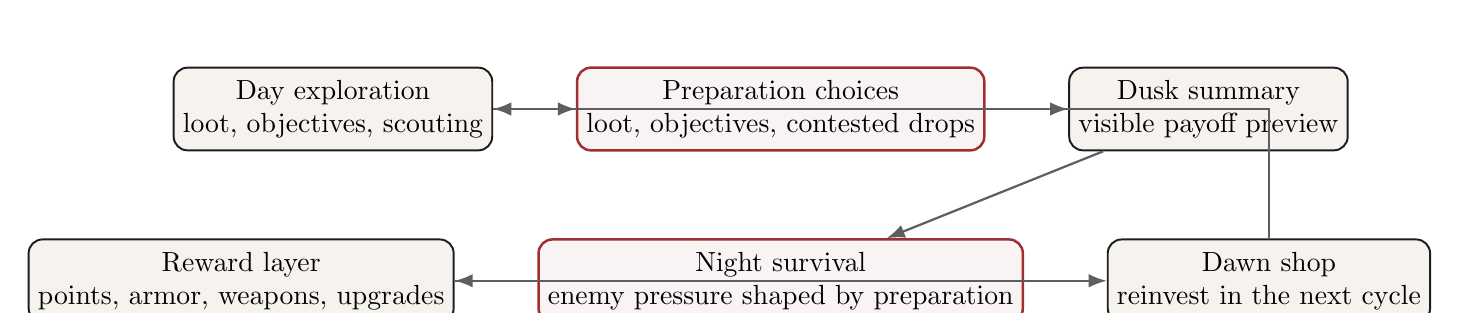
\begin{tikzpicture}[
        node distance=1.1cm and 1.05cm,
        box/.style={
            rectangle,
            rounded corners=5pt,
            draw=deadink,
            line width=0.7pt,
            fill=deadlight,
            align=center,
            minimum width=3.1cm,
            minimum height=1.05cm
        },
        accent/.style={
            rectangle,
            rounded corners=5pt,
            draw=deadred,
            line width=0.9pt,
            fill=deadred!6,
            align=center,
            minimum width=3.1cm,
            minimum height=1.05cm
        },
        arrow/.style={-{Latex[length=2.3mm]}, thick, draw=deadgray}
    ]
        \node[box] (day) {Day exploration\\loot, objectives, scouting};
        \node[accent, right=of day] (prep) {Preparation choices\\loot, objectives, contested drops};
        \node[box, right=of prep] (dusk) {Dusk summary\\visible payoff preview};
        \node[accent, below=of prep] (night) {Night survival\\enemy pressure shaped by preparation};
        \node[box, left=of night] (reward) {Reward layer\\points, armor, weapons, upgrades};
        \node[box, right=of night] (dawn) {Dawn shop\\reinvest in the next cycle};

        \draw[arrow] (day) -- (prep);
        \draw[arrow] (prep) -- (dusk);
        \draw[arrow] (dusk) -- (night);
        \draw[arrow] (night) -- (reward);
        \draw[arrow] (reward) -- (dawn);
        \draw[arrow] (dawn) |- (day);
    \end{tikzpicture}
    }
    \caption{Core Deliverable 2 risk-reward loop. Daytime choices are designed to produce visible nighttime consequences, which then feed into rewards and future preparation.}
\end{figure}

\section{Progression Systems and Rewards}

Progression in the Deliverable 2 prototype works at two levels. The short-term loop is the day-night-dawn cycle within a single mission segment. The long-term loop is the full six-night run across Levels 1 and 2. Together, these systems give the player both immediate rewards and a broader sense of forward movement.

Short-term progression is visible every day. The player gathers resources, earns points, completes objectives, and reaches the dawn shop with a new set of choices. Long-term progression appears across the full prototype route through level unlocks, challenge escalation, and narrative advancement from the Town Center to the Suburban district.

Visible rewards are intentionally mixed:

\begin{itemize}
    \item \textbf{Intrinsic rewards:} better routing, stronger survival discipline, and improved mastery of the game's systems.
    \item \textbf{Extrinsic rewards:} points, weapon access, armor, mission rewards, contested drop bundles, and upgrade purchases.
    \item \textbf{Narrative rewards:} logs, mission context, and story discoveries that make exploration feel worthwhile even when no direct combat reward is attached.
\end{itemize}

Keeping Level 2 in the prototype is important for this reason. It demonstrates unlock-based campaign continuity rather than a single isolated map. After Level 1 is cleared, Level 2 becomes available for manual selection from the menu. Each level begins as a clean deployment state, which keeps difficulty comparisons fair and readable in a prototype context.

\begin{figure}[H]
    \centering
    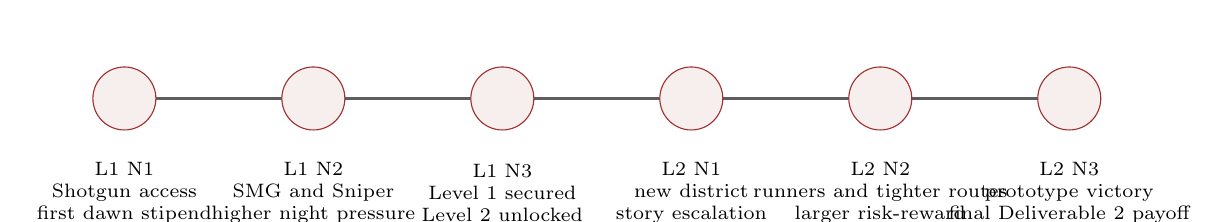
\begin{tikzpicture}[
        milestone/.style={
            circle,
            draw=deadred,
            fill=deadred!8,
            minimum size=8mm,
            inner sep=0pt,
            font=\small\bfseries
        },
        label/.style={align=center, font=\scriptsize},
        line/.style={line width=1.1pt, draw=deadgray}
    ]
        \draw[line] (0,0) -- (12,0);
        \node[milestone] at (0,0) {};
        \node[label] at (0,-1.2) {L1 N1\\Shotgun access\\first dawn stipend};

        \node[milestone] at (2.4,0) {};
        \node[label] at (2.4,-1.2) {L1 N2\\SMG and Sniper\\higher night pressure};

        \node[milestone] at (4.8,0) {};
        \node[label] at (4.8,-1.2) {L1 N3\\Level 1 secured\\Level 2 unlocked};

        \node[milestone] at (7.2,0) {};
        \node[label] at (7.2,-1.2) {L2 N1\\new district\\story escalation};

        \node[milestone] at (9.6,0) {};
        \node[label] at (9.6,-1.2) {L2 N2\\runners and tighter routes\\larger risk-reward};

        \node[milestone] at (12,0) {};
        \node[label] at (12,-1.2) {L2 N3\\prototype victory\\final Deliverable 2 payoff};
    \end{tikzpicture}
    \caption{Six-night progression arc used in the Deliverable 2 build. The second level is important because it gives the prototype a visible campaign structure rather than a single-level slice.}
\end{figure}

\textbf{Implementation detail by point.}
\begin{itemize}
    \item \textbf{Clear unlock rule:} Level 2 access is gated by Level 1 completion to make campaign order explicit.
    \item \textbf{Manual deployment control:} progression does not force auto-jump; players choose when to deploy the next unlocked level.
    \item \textbf{Reward cadence:} every day-night step provides spend/prepare feedback, while level completion provides a larger milestone reward.
    \item \textbf{Fresh-start consistency:} per-level starts are intentionally clean so balance observations are not skewed by cross-level stat carryover.
\end{itemize}

\section{Testing and Iteration}

The prototype was improved through both observation-based feedback and automated runtime validation. Earlier testing suggested that the overall premise was understandable, but that some of the specific story details and system links were not always clear to players on first contact. In response, the design was revised to make communication more direct.

Several changes came from this process. Radio dialogue was strengthened so that the player received more direct context about the situation and the current objective. Mission framing was improved so that important tasks were easier to read. On the systems side, pickup hints, objective panel readability, reward messaging, and dusk summaries were refined so that the player could better understand what had been gained during the day and why it mattered at night.

Systems iteration focused on clarity and fairness. The goal was not only to make mechanics functional, but also to ensure that players could understand them quickly and respond to them with informed decisions. This is especially important in a prototype, where the player must be able to recognize the intended design value of each system without needing extensive explanation outside the game.

\begin{table}[H]
    \centering
    \small
    \begin{tabularx}{\textwidth}{>{\bfseries}p{0.29\textwidth} Y}
        \toprule
        Validation Area & Evidence Included in the Current Prototype \\
        \midrule
        Objective readability & Objective title/status presentation and marker behavior were iterated to reduce overlap and missed-task confusion. \\
        Narrative readability & Speaker/channel labeling and compact COMMS presentation were revised for faster recognition during combat. \\
        Resource clarity & Pickup purpose hints and reward messaging were added to reduce confusion after looting. \\
        Balance response & Night escalation and objective-outcome penalties were tuned to make cause-and-effect legible to players. \\
        Progression behavior & Level completion, unlock gating, and manual next-level selection were tested to ensure predictable campaign flow. \\
        Regression safety & Narrative playtest notes and local PlayMode checks were used to re-verify phase transitions and core loop stability. \\
        \bottomrule
    \end{tabularx}
        \caption{Testing and iteration summary for Deliverable 2. Local PlayMode checks were used as regression evidence for the systems-focused prototype slice.}
\end{table}

\textbf{Implementation detail by point.}
\begin{itemize}
    \item \textbf{Observation-to-fix cycle:} each test pass focused on a player-facing confusion point (e.g., UI overlap, unclear objective state, communication clutter).
    \item \textbf{Low-cost iteration:} most fixes were done at HUD/layout/trigger layers, allowing quick validation without large architectural rewrites.
    \item \textbf{Prototype reliability:} high-risk transitions (day to night, night to dawn, level completion, and death/victory) were repeatedly rechecked after each UI/system revision.
\end{itemize}

\section{Technical Notes}

Several Unity systems supported this iteration:

\begin{itemize}
    \item \textbf{Game flow and campaign state:} \texttt{GameManager} and \texttt{GameFlowController} coordinate the day, night, dawn, and level transition structure.
    \item \textbf{Mission guidance:} \texttt{StoryObjective}, the objective HUD, and objective markers provide in-world direction without relying on a heavy tutorial layer.
    \item \textbf{Narrative support:} radio updates, mission scripting, and lore systems support layered story delivery across the run.
    \item \textbf{Balance and preparation systems:} \texttt{SupplyCrate}, \texttt{Pickup}, \texttt{PointsSystem}, and the wave balancing path connect day preparation to night pressure.
    \item \textbf{Current feature gating:} crafting hooks exist in code but are disabled in this Deliverable 2 build (\texttt{enableCrafting = false}) to keep the prototype loop clean and readable.
    \item \textbf{Submission structure:} the Deliverable 2 package is organized around the Unity project, the standalone build output, and this written PDF report.
\end{itemize}

\section{Upcoming Deliverable 3 Implementations}

The next milestone is planned as an expansion pass rather than a redesign. The current Deliverable 2 prototype establishes a stable baseline (Levels 1-2, manual level selection, and per-level fresh starts). Deliverable 3 will extend this baseline in the following areas:

\begin{itemize}
    \item \textbf{Playable scope expansion:} unlock and ship Levels 3 and 4, with Industrial and Research spaces fully integrated into the campaign route.
    \item \textbf{Final-stage encounters:} add late-campaign pressure patterns and final-encounter tuning for the Level 4 end-state.
    \item \textbf{Narrative continuity upgrade:} add level-specific transmissions and objective chains for Levels 3-4 so progression feels authored end-to-end.
    \item \textbf{System depth pass:} revisit optional advanced preparation systems (including potential crafting return) only if readability and clutter targets remain satisfied.
    \item \textbf{Progression quality-of-life:} add clearer run-state communication (resume vs restart intent), additional end-of-level feedback, and stronger scoreboard/run-summary clarity.
    \item \textbf{Validation scope increase:} broaden regression coverage around level transitions, late-game balance, and ending flows after the full four-level route is enabled.
\end{itemize}

\section{Conclusion}

Deliverable 2 represents a clear step forward from a basic survival prototype to a more cohesive game experience. The current build demonstrates readable level flow, stronger player guidance, clearer narrative integration, more understandable systems balancing, and a progression structure that benefits from spanning two linked levels instead of one isolated map.

Most importantly, the project's mechanics now support the setting and the intended player experience. The player is not only surviving enemy waves. They are exploring for resources, following mission leads, reacting to radio updates, and seeing how preparation, pressure, and reward connect across the campaign. This integration is the main achievement of the Deliverable 2 build and provides a strong foundation for future deliverables.

\end{document}
